\documentclass[1p]{elsarticle_modified}
%\bibliographystyle{elsarticle-num}

%\usepackage[colorlinks]{hyperref}
%\usepackage{abbrmath_seonhwa} %\Abb, \Ascr, \Acal ,\Abf, \Afrak
\usepackage{amsfonts}
\usepackage{amssymb}
\usepackage{amsmath}
\usepackage{amsthm}
\usepackage{scalefnt}
\usepackage{amsbsy}
\usepackage{kotex}
\usepackage{caption}
\usepackage{subfig}
\usepackage{color}
\usepackage{graphicx}
\usepackage{xcolor} %% white, black, red, green, blue, cyan, magenta, yellow
\usepackage{float}
\usepackage{setspace}
\usepackage{hyperref}

\usepackage{tikz}
\usetikzlibrary{arrows}

\usepackage{multirow}
\usepackage{array} % fixed length table
\usepackage{hhline}

%%%%%%%%%%%%%%%%%%%%%
\makeatletter
\renewcommand*\env@matrix[1][\arraystretch]{%
	\edef\arraystretch{#1}%
	\hskip -\arraycolsep
	\let\@ifnextchar\new@ifnextchar
	\array{*\c@MaxMatrixCols c}}
\makeatother %https://tex.stackexchange.com/questions/14071/how-can-i-increase-the-line-spacing-in-a-matrix
%%%%%%%%%%%%%%%

\usepackage[normalem]{ulem}

\newcommand{\msout}[1]{\ifmmode\text{\sout{\ensuremath{#1}}}\else\sout{#1}\fi}
%SOURCE: \msout is \stkout macro in https://tex.stackexchange.com/questions/20609/strikeout-in-math-mode

\newcommand{\cancel}[1]{
	\ifmmode
	{\color{red}\msout{#1}}
	\else
	{\color{red}\sout{#1}}
	\fi
}

\newcommand{\add}[1]{
	{\color{blue}\uwave{#1}}
}

\newcommand{\replace}[2]{
	\ifmmode
	{\color{red}\msout{#1}}{\color{blue}\uwave{#2}}
	\else
	{\color{red}\sout{#1}}{\color{blue}\uwave{#2}}
	\fi
}

\newcommand{\Sol}{\mathcal{S}} %segment
\newcommand{\D}{D} %diagram
\newcommand{\A}{\mathcal{A}} %arc


%%%%%%%%%%%%%%%%%%%%%%%%%%%%%5 test

\def\sl{\operatorname{\textup{SL}}(2,\Cbb)}
\def\psl{\operatorname{\textup{PSL}}(2,\Cbb)}
\def\quan{\mkern 1mu \triangleright \mkern 1mu}

\theoremstyle{definition}
\newtheorem{thm}{Theorem}[section]
\newtheorem{prop}[thm]{Proposition}
\newtheorem{lem}[thm]{Lemma}
\newtheorem{ques}[thm]{Question}
\newtheorem{cor}[thm]{Corollary}
\newtheorem{defn}[thm]{Definition}
\newtheorem{exam}[thm]{Example}
\newtheorem{rmk}[thm]{Remark}
\newtheorem{alg}[thm]{Algorithm}

\newcommand{\I}{\sqrt{-1}}
\begin{document}

%\begin{frontmatter}
%
%\title{Boundary parabolic representations of knots up to 8 crossings}
%
%%% Group authors per affiliation:
%\author{Yunhi Cho} 
%\address{Department of Mathematics, University of Seoul, Seoul, Korea}
%\ead{yhcho@uos.ac.kr}
%
%
%\author{Seonhwa Kim} %\fnref{s_kim}}
%\address{Center for Geometry and Physics, Institute for Basic Science, Pohang, 37673, Korea}
%\ead{ryeona17@ibs.re.kr}
%
%\author{Hyuk Kim}
%\address{Department of Mathematical Sciences, Seoul National University, Seoul 08826, Korea}
%\ead{hyukkim@snu.ac.kr}
%
%\author{Seokbeom Yoon}
%\address{Department of Mathematical Sciences, Seoul National University, Seoul, 08826,  Korea}
%\ead{sbyoon15@snu.ac.kr}
%
%\begin{abstract}
%We find all boundary parabolic representation of knots up to 8 crossings.
%
%\end{abstract}
%\begin{keyword}
%    \MSC[2010] 57M25 
%\end{keyword}
%
%\end{frontmatter}

%\linenumbers
%\tableofcontents
%
\newcommand\colored[1]{\textcolor{white}{\rule[-0.35ex]{0.8em}{1.4ex}}\kern-0.8em\color{red} #1}%
%\newcommand\colored[1]{\textcolor{white}{ #1}\kern-2.17ex	\textcolor{white}{ #1}\kern-1.81ex	\textcolor{white}{ #1}\kern-2.15ex\color{red}#1	}

{\Large $\underline{12a_{0342}~(K12a_{0342})}$}

\setlength{\tabcolsep}{10pt}
\renewcommand{\arraystretch}{1.6}
\vspace{1cm}\begin{tabular}{m{100pt}>{\centering\arraybackslash}m{274pt}}
\multirow{5}{120pt}{
	\centering
	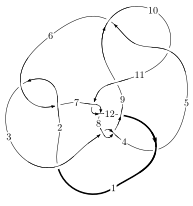
\includegraphics[width=112pt]{../../../GIT/diagram.site/Diagrams/png/1143_12a_0342.png}\\
\ \ \ A knot diagram\footnotemark}&
\allowdisplaybreaks
\textbf{Linearized knot diagam} \\
\cline{2-2}
 &
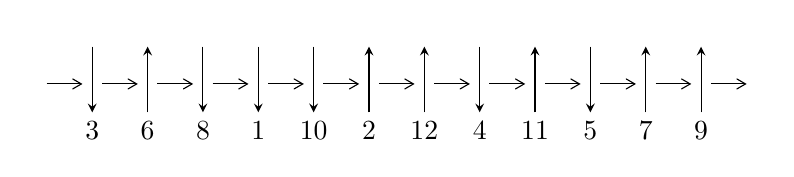
\begin{tikzpicture}[x=20pt, y=17pt]
	% nodes
	\node (C0) at (0, 0) {};
	\node (C1) at (1, 0) {};
	\node (C1U) at (1, +1) {};
	\node (C1D) at (1, -1) {3};

	\node (C2) at (2, 0) {};
	\node (C2U) at (2, +1) {};
	\node (C2D) at (2, -1) {6};

	\node (C3) at (3, 0) {};
	\node (C3U) at (3, +1) {};
	\node (C3D) at (3, -1) {8};

	\node (C4) at (4, 0) {};
	\node (C4U) at (4, +1) {};
	\node (C4D) at (4, -1) {1};

	\node (C5) at (5, 0) {};
	\node (C5U) at (5, +1) {};
	\node (C5D) at (5, -1) {10};

	\node (C6) at (6, 0) {};
	\node (C6U) at (6, +1) {};
	\node (C6D) at (6, -1) {2};

	\node (C7) at (7, 0) {};
	\node (C7U) at (7, +1) {};
	\node (C7D) at (7, -1) {12};

	\node (C8) at (8, 0) {};
	\node (C8U) at (8, +1) {};
	\node (C8D) at (8, -1) {4};

	\node (C9) at (9, 0) {};
	\node (C9U) at (9, +1) {};
	\node (C9D) at (9, -1) {11};

	\node (C10) at (10, 0) {};
	\node (C10U) at (10, +1) {};
	\node (C10D) at (10, -1) {5};

	\node (C11) at (11, 0) {};
	\node (C11U) at (11, +1) {};
	\node (C11D) at (11, -1) {7};

	\node (C12) at (12, 0) {};
	\node (C12U) at (12, +1) {};
	\node (C12D) at (12, -1) {9};
	\node (C13) at (13, 0) {};

	% arrows
	\draw[->,>={angle 60}]
	(C0) edge (C1) (C1) edge (C2) (C2) edge (C3) (C3) edge (C4) (C4) edge (C5) (C5) edge (C6) (C6) edge (C7) (C7) edge (C8) (C8) edge (C9) (C9) edge (C10) (C10) edge (C11) (C11) edge (C12) (C12) edge (C13) ;	\draw[->,>=stealth]
	(C1U) edge (C1D) (C2D) edge (C2U) (C3U) edge (C3D) (C4U) edge (C4D) (C5U) edge (C5D) (C6D) edge (C6U) (C7D) edge (C7U) (C8U) edge (C8D) (C9D) edge (C9U) (C10U) edge (C10D) (C11D) edge (C11U) (C12D) edge (C12U) ;
	\end{tikzpicture} \\
\hhline{~~} \\& 
\textbf{Solving Sequence} \\ \cline{2-2} 
 &
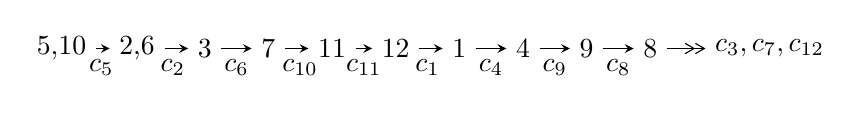
\begin{tikzpicture}[x=23pt, y=7pt]
	% node
	\node (A0) at (-1/8, 0) {5,10};
	\node (A1) at (17/16, 0) {2,6};
	\node (A2) at (17/8, 0) {3};
	\node (A3) at (25/8, 0) {7};
	\node (A4) at (33/8, 0) {11};
	\node (A5) at (41/8, 0) {12};
	\node (A6) at (49/8, 0) {1};
	\node (A7) at (57/8, 0) {4};
	\node (A8) at (65/8, 0) {9};
	\node (A9) at (73/8, 0) {8};
	\node (C1) at (1/2, -1) {$c_{5}$};
	\node (C2) at (13/8, -1) {$c_{2}$};
	\node (C3) at (21/8, -1) {$c_{6}$};
	\node (C4) at (29/8, -1) {$c_{10}$};
	\node (C5) at (37/8, -1) {$c_{11}$};
	\node (C6) at (45/8, -1) {$c_{1}$};
	\node (C7) at (53/8, -1) {$c_{4}$};
	\node (C8) at (61/8, -1) {$c_{9}$};
	\node (C9) at (69/8, -1) {$c_{8}$};
	\node (A10) at (11, 0) {$c_{3},c_{7},c_{12}$};

	% edge
	\draw[->,>=stealth]	
	(A0) edge (A1) (A1) edge (A2) (A2) edge (A3) (A3) edge (A4) (A4) edge (A5) (A5) edge (A6) (A6) edge (A7) (A7) edge (A8) (A8) edge (A9) ;
	\draw[->>,>={angle 60}]	
	(A9) edge (A10);
\end{tikzpicture} \\ 

\end{tabular} \\

\footnotetext{
The image of knot diagram is generated by the software ``\textbf{Draw programme}" developed by Andrew Bartholomew(\url{http://www.layer8.co.uk/maths/draw/index.htm\#Running-draw}), where we modified some parts for our purpose(\url{https://github.com/CATsTAILs/LinksPainter}).
}\phantom \\ \newline 
\centering \textbf{Ideals for irreducible components\footnotemark of $X_{\text{par}}$} 
 
\begin{align*}
I^u_{1}&=\langle 
-1.20197\times10^{404} u^{155}-1.98407\times10^{404} u^{154}+\cdots+1.03297\times10^{404} b-1.24809\times10^{407},\\
\phantom{I^u_{1}}&\phantom{= \langle  }-2.63389\times10^{406} u^{155}+8.44260\times10^{406} u^{154}+\cdots+7.75764\times10^{406} a+6.28696\times10^{409},\\
\phantom{I^u_{1}}&\phantom{= \langle  }u^{156}+u^{155}+\cdots-643 u+751\rangle \\
I^u_{2}&=\langle 
-7283 u^{37}+6235 u^{36}+\cdots+995 b-2491,\;3092 u^{37}-2046 u^{36}+\cdots+995 a+12148,\\
\phantom{I^u_{2}}&\phantom{= \langle  }u^{38}+12 u^{36}+\cdots+2 u+1\rangle \\
\\
\end{align*}
\raggedright * 2 irreducible components of $\dim_{\mathbb{C}}=0$, with total 194 representations.\\
\footnotetext{All coefficients of polynomials are rational numbers. But the coefficients are sometimes approximated in decimal forms when there is not enough margin.}
\newpage
\renewcommand{\arraystretch}{1}
\centering \section*{I. $I^u_{1}= \langle -1.20\times10^{404} u^{155}-1.98\times10^{404} u^{154}+\cdots+1.03\times10^{404} b-1.25\times10^{407},\;-2.63\times10^{406} u^{155}+8.44\times10^{406} u^{154}+\cdots+7.76\times10^{406} a+6.29\times10^{409},\;u^{156}+u^{155}+\cdots-643 u+751 \rangle$}
\flushleft \textbf{(i) Arc colorings}\\
\begin{tabular}{m{7pt} m{180pt} m{7pt} m{180pt} }
\flushright $a_{5}=$&$\begin{pmatrix}1\\0\end{pmatrix}$ \\
\flushright $a_{10}=$&$\begin{pmatrix}0\\u\end{pmatrix}$ \\
\flushright $a_{2}=$&$\begin{pmatrix}0.339523 u^{155}-1.08830 u^{154}+\cdots+1312.04 u-810.422\\1.16361 u^{155}+1.92074 u^{154}+\cdots-990.348 u+1208.25\end{pmatrix}$ \\
\flushright $a_{6}=$&$\begin{pmatrix}1\\u^2\end{pmatrix}$ \\
\flushright $a_{3}=$&$\begin{pmatrix}0.887263 u^{155}-0.732362 u^{154}+\cdots+1494.76 u-674.462\\0.803609 u^{155}+1.94703 u^{154}+\cdots-1525.03 u+1352.30\end{pmatrix}$ \\
\flushright $a_{7}=$&$\begin{pmatrix}0.240562 u^{155}+0.684041 u^{154}+\cdots-624.185 u+655.447\\-0.222710 u^{155}-1.77408 u^{154}+\cdots+1850.31 u-1384.20\end{pmatrix}$ \\
\flushright $a_{11}=$&$\begin{pmatrix}- u\\u\end{pmatrix}$ \\
\flushright $a_{12}=$&$\begin{pmatrix}1.58683 u^{155}-2.09974 u^{154}+\cdots+4195.43 u-1967.02\\-0.323186 u^{155}+3.07800 u^{154}+\cdots-4460.22 u+2614.13\end{pmatrix}$ \\
\flushright $a_{1}=$&$\begin{pmatrix}-0.724223 u^{155}-4.21579 u^{154}+\cdots+3923.98 u-2938.41\\0.518971 u^{155}+2.43169 u^{154}+\cdots-2514.80 u+1834.96\end{pmatrix}$ \\
\flushright $a_{4}=$&$\begin{pmatrix}0.363334 u^{155}-0.0490247 u^{154}+\cdots+370.041 u+97.1690\\0.721342 u^{155}+2.37469 u^{154}+\cdots-1453.60 u+1335.56\end{pmatrix}$ \\
\flushright $a_{9}=$&$\begin{pmatrix}- u^3\\u^3+u\end{pmatrix}$ \\
\flushright $a_{8}=$&$\begin{pmatrix}0.428023 u^{155}-1.47511 u^{154}+\cdots+2752.95 u-1358.47\\0.845539 u^{155}+0.990339 u^{154}+\cdots-279.843 u+478.958\end{pmatrix}$\\&\end{tabular}
\flushleft \textbf{(ii) Obstruction class $= -1$}\\~\\
\flushleft \textbf{(iii) Cusp Shapes $= -6.61247 u^{155}-7.18823 u^{154}+\cdots-439.660 u-3074.15$}\\~\\
\newpage\renewcommand{\arraystretch}{1}
\flushleft \textbf{(iv) u-Polynomials at the component}\newline \\
\begin{tabular}{m{50pt}|m{274pt}}
Crossings & \hspace{64pt}u-Polynomials at each crossing \\
\hline $$\begin{aligned}c_{1}\end{aligned}$$&$\begin{aligned}
&u^{156}+68 u^{155}+\cdots+586213058 u+32137561
\end{aligned}$\\
\hline $$\begin{aligned}c_{2},c_{6}\end{aligned}$$&$\begin{aligned}
&u^{156}-2 u^{155}+\cdots-17042 u+5669
\end{aligned}$\\
\hline $$\begin{aligned}c_{3},c_{8}\end{aligned}$$&$\begin{aligned}
&u^{156}- u^{155}+\cdots+6147 u+2449
\end{aligned}$\\
\hline $$\begin{aligned}c_{4}\end{aligned}$$&$\begin{aligned}
&u^{156}-4 u^{155}+\cdots-513066 u+23269
\end{aligned}$\\
\hline $$\begin{aligned}c_{5},c_{10}\end{aligned}$$&$\begin{aligned}
&u^{156}- u^{155}+\cdots+643 u+751
\end{aligned}$\\
\hline $$\begin{aligned}c_{7},c_{11}\end{aligned}$$&$\begin{aligned}
&u^{156}-3 u^{155}+\cdots+107845 u+85523
\end{aligned}$\\
\hline $$\begin{aligned}c_{9}\end{aligned}$$&$\begin{aligned}
&u^{156}-77 u^{155}+\cdots-10171145 u+564001
\end{aligned}$\\
\hline $$\begin{aligned}c_{12}\end{aligned}$$&$\begin{aligned}
&u^{156}+9 u^{155}+\cdots-1045 u+521
\end{aligned}$\\
\hline
\end{tabular}\\~\\
\newpage\renewcommand{\arraystretch}{1}
\flushleft \textbf{(v) Riley Polynomials at the component}\newline \\
\begin{tabular}{m{50pt}|m{274pt}}
Crossings & \hspace{64pt}Riley Polynomials at each crossing \\
\hline $$\begin{aligned}c_{1}\end{aligned}$$&$\begin{aligned}
&y^{156}+60 y^{155}+\cdots+29158613325391790 y+1032822827028721
\end{aligned}$\\
\hline $$\begin{aligned}c_{2},c_{6}\end{aligned}$$&$\begin{aligned}
&y^{156}+68 y^{155}+\cdots+586213058 y+32137561
\end{aligned}$\\
\hline $$\begin{aligned}c_{3},c_{8}\end{aligned}$$&$\begin{aligned}
&y^{156}-83 y^{155}+\cdots-131376593 y+5997601
\end{aligned}$\\
\hline $$\begin{aligned}c_{4}\end{aligned}$$&$\begin{aligned}
&y^{156}-20 y^{155}+\cdots-25116154598 y+541446361
\end{aligned}$\\
\hline $$\begin{aligned}c_{5},c_{10}\end{aligned}$$&$\begin{aligned}
&y^{156}+77 y^{155}+\cdots+10171145 y+564001
\end{aligned}$\\
\hline $$\begin{aligned}c_{7},c_{11}\end{aligned}$$&$\begin{aligned}
&y^{156}-105 y^{155}+\cdots+830770663883 y+7314183529
\end{aligned}$\\
\hline $$\begin{aligned}c_{9}\end{aligned}$$&$\begin{aligned}
&y^{156}+25 y^{155}+\cdots+20263498622645 y+318097128001
\end{aligned}$\\
\hline $$\begin{aligned}c_{12}\end{aligned}$$&$\begin{aligned}
&y^{156}+11 y^{155}+\cdots+19725051 y+271441
\end{aligned}$\\
\hline
\end{tabular}\\~\\
\newpage\flushleft \textbf{(vi) Complex Volumes and Cusp Shapes}
$$\begin{array}{c|c|c}  
\text{Solutions to }I^u_{1}& \I (\text{vol} + \sqrt{-1}CS) & \text{Cusp shape}\\
 \hline 
\begin{aligned}
u &= \phantom{-}0.314686 + 0.948049 I \\
a &= -1.122900 + 0.399488 I \\
b &= -0.05478 - 1.90960 I\end{aligned}
 & \phantom{-}4.50020 + 0.21846 I & \phantom{-0.000000 } 0 \\ \hline\begin{aligned}
u &= \phantom{-}0.314686 - 0.948049 I \\
a &= -1.122900 - 0.399488 I \\
b &= -0.05478 + 1.90960 I\end{aligned}
 & \phantom{-}4.50020 - 0.21846 I & \phantom{-0.000000 } 0 \\ \hline\begin{aligned}
u &= -0.170790 + 0.987084 I \\
a &= \phantom{-}0.633623 - 1.049930 I \\
b &= -0.357628 + 0.104624 I\end{aligned}
 & \phantom{-}3.20120 - 1.52428 I & \phantom{-0.000000 } 0 \\ \hline\begin{aligned}
u &= -0.170790 - 0.987084 I \\
a &= \phantom{-}0.633623 + 1.049930 I \\
b &= -0.357628 - 0.104624 I\end{aligned}
 & \phantom{-}3.20120 + 1.52428 I & \phantom{-0.000000 } 0 \\ \hline\begin{aligned}
u &= -0.389580 + 0.925758 I \\
a &= -3.06881 + 1.42393 I \\
b &= \phantom{-}2.74803 + 0.41625 I\end{aligned}
 & -0.36759 - 1.52334 I & \phantom{-0.000000 } 0 \\ \hline\begin{aligned}
u &= -0.389580 - 0.925758 I \\
a &= -3.06881 - 1.42393 I \\
b &= \phantom{-}2.74803 - 0.41625 I\end{aligned}
 & -0.36759 + 1.52334 I & \phantom{-0.000000 } 0 \\ \hline\begin{aligned}
u &= \phantom{-}0.764967 + 0.665148 I \\
a &= \phantom{-}0.30131 + 1.97652 I \\
b &= -1.77763 - 0.59009 I\end{aligned}
 & -8.04521 - 0.38455 I & \phantom{-0.000000 } 0 \\ \hline\begin{aligned}
u &= \phantom{-}0.764967 - 0.665148 I \\
a &= \phantom{-}0.30131 - 1.97652 I \\
b &= -1.77763 + 0.59009 I\end{aligned}
 & -8.04521 + 0.38455 I & \phantom{-0.000000 } 0 \\ \hline\begin{aligned}
u &= -0.287570 + 0.978275 I \\
a &= \phantom{-}1.141850 - 0.391800 I \\
b &= -0.447530 - 1.222970 I\end{aligned}
 & \phantom{-}4.40725 - 3.47807 I & \phantom{-0.000000 } 0 \\ \hline\begin{aligned}
u &= -0.287570 - 0.978275 I \\
a &= \phantom{-}1.141850 + 0.391800 I \\
b &= -0.447530 + 1.222970 I\end{aligned}
 & \phantom{-}4.40725 + 3.47807 I & \phantom{-0.000000 } 0\\
 \hline 
 \end{array}$$\newpage$$\begin{array}{c|c|c}  
\text{Solutions to }I^u_{1}& \I (\text{vol} + \sqrt{-1}CS) & \text{Cusp shape}\\
 \hline 
\begin{aligned}
u &= \phantom{-}0.379406 + 0.964078 I \\
a &= \phantom{-}2.31237 + 1.11954 I \\
b &= -2.06980 - 0.13247 I\end{aligned}
 & \phantom{-}2.40104 - 3.09117 I & \phantom{-0.000000 } 0 \\ \hline\begin{aligned}
u &= \phantom{-}0.379406 - 0.964078 I \\
a &= \phantom{-}2.31237 - 1.11954 I \\
b &= -2.06980 + 0.13247 I\end{aligned}
 & \phantom{-}2.40104 + 3.09117 I & \phantom{-0.000000 } 0 \\ \hline\begin{aligned}
u &= \phantom{-}0.168715 + 0.947032 I \\
a &= -0.609414 - 0.921753 I \\
b &= \phantom{-}0.157383 + 0.470877 I\end{aligned}
 & \phantom{-}1.28269 - 2.51191 I & \phantom{-0.000000 } 0 \\ \hline\begin{aligned}
u &= \phantom{-}0.168715 - 0.947032 I \\
a &= -0.609414 + 0.921753 I \\
b &= \phantom{-}0.157383 - 0.470877 I\end{aligned}
 & \phantom{-}1.28269 + 2.51191 I & \phantom{-0.000000 } 0 \\ \hline\begin{aligned}
u &= -0.620529 + 0.727479 I \\
a &= \phantom{-}0.916688 + 0.299057 I \\
b &= \phantom{-}0.575110 - 0.684533 I\end{aligned}
 & -2.52818 + 5.31514 I & \phantom{-0.000000 } 0 \\ \hline\begin{aligned}
u &= -0.620529 - 0.727479 I \\
a &= \phantom{-}0.916688 - 0.299057 I \\
b &= \phantom{-}0.575110 + 0.684533 I\end{aligned}
 & -2.52818 - 5.31514 I & \phantom{-0.000000 } 0 \\ \hline\begin{aligned}
u &= -0.192813 + 1.026250 I \\
a &= -0.1149880 - 0.0450683 I \\
b &= -0.211794 + 1.044400 I\end{aligned}
 & -1.75492 - 0.21945 I & \phantom{-0.000000 } 0 \\ \hline\begin{aligned}
u &= -0.192813 - 1.026250 I \\
a &= -0.1149880 + 0.0450683 I \\
b &= -0.211794 - 1.044400 I\end{aligned}
 & -1.75492 + 0.21945 I & \phantom{-0.000000 } 0 \\ \hline\begin{aligned}
u &= -0.967091 + 0.396088 I \\
a &= -0.07366 + 1.60101 I \\
b &= \phantom{-}1.82974 + 0.15178 I\end{aligned}
 & -2.07204 - 13.90080 I & \phantom{-0.000000 } 0 \\ \hline\begin{aligned}
u &= -0.967091 - 0.396088 I \\
a &= -0.07366 - 1.60101 I \\
b &= \phantom{-}1.82974 - 0.15178 I\end{aligned}
 & -2.07204 + 13.90080 I & \phantom{-0.000000 } 0\\
 \hline 
 \end{array}$$\newpage$$\begin{array}{c|c|c}  
\text{Solutions to }I^u_{1}& \I (\text{vol} + \sqrt{-1}CS) & \text{Cusp shape}\\
 \hline 
\begin{aligned}
u &= -0.310213 + 0.900109 I \\
a &= -1.06413 + 1.58543 I \\
b &= \phantom{-}1.97565 - 1.89639 I\end{aligned}
 & -2.43039 - 4.42948 I & \phantom{-0.000000 } 0 \\ \hline\begin{aligned}
u &= -0.310213 - 0.900109 I \\
a &= -1.06413 - 1.58543 I \\
b &= \phantom{-}1.97565 + 1.89639 I\end{aligned}
 & -2.43039 + 4.42948 I & \phantom{-0.000000 } 0 \\ \hline\begin{aligned}
u &= -0.522391 + 0.912570 I \\
a &= -0.575948 + 0.066149 I \\
b &= -0.085719 + 1.120830 I\end{aligned}
 & -1.95927 - 0.77778 I & \phantom{-0.000000 } 0 \\ \hline\begin{aligned}
u &= -0.522391 - 0.912570 I \\
a &= -0.575948 - 0.066149 I \\
b &= -0.085719 - 1.120830 I\end{aligned}
 & -1.95927 + 0.77778 I & \phantom{-0.000000 } 0 \\ \hline\begin{aligned}
u &= -0.909221 + 0.259472 I \\
a &= \phantom{-}0.123111 + 0.685530 I \\
b &= -0.316398 + 0.008844 I\end{aligned}
 & \phantom{-}2.89929 - 2.34324 I & \phantom{-0.000000 } 0 \\ \hline\begin{aligned}
u &= -0.909221 - 0.259472 I \\
a &= \phantom{-}0.123111 - 0.685530 I \\
b &= -0.316398 - 0.008844 I\end{aligned}
 & \phantom{-}2.89929 + 2.34324 I & \phantom{-0.000000 } 0 \\ \hline\begin{aligned}
u &= \phantom{-}0.327121 + 0.886426 I \\
a &= \phantom{-}0.21564 + 2.15420 I \\
b &= -1.73820 - 2.40526 I\end{aligned}
 & \phantom{-}2.00818 + 0.26275 I & \phantom{-0.000000 } 0 \\ \hline\begin{aligned}
u &= \phantom{-}0.327121 - 0.886426 I \\
a &= \phantom{-}0.21564 - 2.15420 I \\
b &= -1.73820 + 2.40526 I\end{aligned}
 & \phantom{-}2.00818 - 0.26275 I & \phantom{-0.000000 } 0 \\ \hline\begin{aligned}
u &= \phantom{-}0.761910 + 0.558313 I \\
a &= -0.99544 - 1.87431 I \\
b &= \phantom{-}1.142060 - 0.268267 I\end{aligned}
 & -1.75544 + 0.37427 I & \phantom{-0.000000 } 0 \\ \hline\begin{aligned}
u &= \phantom{-}0.761910 - 0.558313 I \\
a &= -0.99544 + 1.87431 I \\
b &= \phantom{-}1.142060 + 0.268267 I\end{aligned}
 & -1.75544 - 0.37427 I & \phantom{-0.000000 } 0\\
 \hline 
 \end{array}$$\newpage$$\begin{array}{c|c|c}  
\text{Solutions to }I^u_{1}& \I (\text{vol} + \sqrt{-1}CS) & \text{Cusp shape}\\
 \hline 
\begin{aligned}
u &= -0.369426 + 0.994086 I \\
a &= -1.96669 + 1.41932 I \\
b &= \phantom{-}2.20930 - 0.98738 I\end{aligned}
 & -1.96143 + 7.05234 I & \phantom{-0.000000 } 0 \\ \hline\begin{aligned}
u &= -0.369426 - 0.994086 I \\
a &= -1.96669 - 1.41932 I \\
b &= \phantom{-}2.20930 + 0.98738 I\end{aligned}
 & -1.96143 - 7.05234 I & \phantom{-0.000000 } 0 \\ \hline\begin{aligned}
u &= -0.231301 + 0.909026 I \\
a &= \phantom{-}0.172950 - 0.756205 I \\
b &= \phantom{-}0.513443 - 0.335586 I\end{aligned}
 & \phantom{-}4.28323 - 1.07875 I & \phantom{-0.000000 } 0 \\ \hline\begin{aligned}
u &= -0.231301 - 0.909026 I \\
a &= \phantom{-}0.172950 + 0.756205 I \\
b &= \phantom{-}0.513443 + 0.335586 I\end{aligned}
 & \phantom{-}4.28323 + 1.07875 I & \phantom{-0.000000 } 0 \\ \hline\begin{aligned}
u &= \phantom{-}0.873648 + 0.340491 I \\
a &= -0.346265 + 0.707821 I \\
b &= \phantom{-}0.281624 - 0.173512 I\end{aligned}
 & \phantom{-}0.13196 + 8.09309 I & \phantom{-0.000000 } 0 \\ \hline\begin{aligned}
u &= \phantom{-}0.873648 - 0.340491 I \\
a &= -0.346265 - 0.707821 I \\
b &= \phantom{-}0.281624 + 0.173512 I\end{aligned}
 & \phantom{-}0.13196 - 8.09309 I & \phantom{-0.000000 } 0 \\ \hline\begin{aligned}
u &= -0.368759 + 0.861294 I \\
a &= -0.21879 + 3.23453 I \\
b &= \phantom{-}2.37621 - 2.72280 I\end{aligned}
 & -0.61701 + 4.67868 I & \phantom{-0.000000 } 0 \\ \hline\begin{aligned}
u &= -0.368759 - 0.861294 I \\
a &= -0.21879 - 3.23453 I \\
b &= \phantom{-}2.37621 + 2.72280 I\end{aligned}
 & -0.61701 - 4.67868 I & \phantom{-0.000000 } 0 \\ \hline\begin{aligned}
u &= \phantom{-}0.324965 + 1.012440 I \\
a &= \phantom{-}1.44767 - 0.05934 I \\
b &= -0.494335 + 0.177695 I\end{aligned}
 & \phantom{-}4.69177 - 2.40977 I & \phantom{-0.000000 } 0 \\ \hline\begin{aligned}
u &= \phantom{-}0.324965 - 1.012440 I \\
a &= \phantom{-}1.44767 + 0.05934 I \\
b &= -0.494335 - 0.177695 I\end{aligned}
 & \phantom{-}4.69177 + 2.40977 I & \phantom{-0.000000 } 0\\
 \hline 
 \end{array}$$\newpage$$\begin{array}{c|c|c}  
\text{Solutions to }I^u_{1}& \I (\text{vol} + \sqrt{-1}CS) & \text{Cusp shape}\\
 \hline 
\begin{aligned}
u &= \phantom{-}0.277751 + 0.894534 I \\
a &= \phantom{-}0.272369 - 0.204315 I \\
b &= -1.045410 - 0.821220 I\end{aligned}
 & \phantom{-}3.59555 + 3.72788 I & \phantom{-0.000000 } 0 \\ \hline\begin{aligned}
u &= \phantom{-}0.277751 - 0.894534 I \\
a &= \phantom{-}0.272369 + 0.204315 I \\
b &= -1.045410 + 0.821220 I\end{aligned}
 & \phantom{-}3.59555 - 3.72788 I & \phantom{-0.000000 } 0 \\ \hline\begin{aligned}
u &= \phantom{-}1.015980 + 0.348748 I \\
a &= -0.03654 + 1.55044 I \\
b &= -1.73438 + 0.30252 I\end{aligned}
 & \phantom{-}1.04423 + 7.45505 I & \phantom{-0.000000 } 0 \\ \hline\begin{aligned}
u &= \phantom{-}1.015980 - 0.348748 I \\
a &= -0.03654 - 1.55044 I \\
b &= -1.73438 - 0.30252 I\end{aligned}
 & \phantom{-}1.04423 - 7.45505 I & \phantom{-0.000000 } 0 \\ \hline\begin{aligned}
u &= \phantom{-}0.214175 + 1.057270 I \\
a &= -0.817825 - 1.130120 I \\
b &= \phantom{-}0.895341 - 0.109395 I\end{aligned}
 & -0.96779 + 5.37139 I & \phantom{-0.000000 } 0 \\ \hline\begin{aligned}
u &= \phantom{-}0.214175 - 1.057270 I \\
a &= -0.817825 + 1.130120 I \\
b &= \phantom{-}0.895341 + 0.109395 I\end{aligned}
 & -0.96779 - 5.37139 I & \phantom{-0.000000 } 0 \\ \hline\begin{aligned}
u &= \phantom{-}0.834858 + 0.385886 I \\
a &= \phantom{-}0.504327 - 1.072800 I \\
b &= \phantom{-}1.30683 + 0.76592 I\end{aligned}
 & -5.07291 - 2.27519 I & \phantom{-0.000000 } 0 \\ \hline\begin{aligned}
u &= \phantom{-}0.834858 - 0.385886 I \\
a &= \phantom{-}0.504327 + 1.072800 I \\
b &= \phantom{-}1.30683 - 0.76592 I\end{aligned}
 & -5.07291 + 2.27519 I & \phantom{-0.000000 } 0 \\ \hline\begin{aligned}
u &= \phantom{-}0.392121 + 1.007210 I \\
a &= \phantom{-}0.884957 + 1.045460 I \\
b &= -0.452494 - 1.041260 I\end{aligned}
 & \phantom{-}4.37259 - 6.31285 I & \phantom{-0.000000 } 0 \\ \hline\begin{aligned}
u &= \phantom{-}0.392121 - 1.007210 I \\
a &= \phantom{-}0.884957 - 1.045460 I \\
b &= -0.452494 + 1.041260 I\end{aligned}
 & \phantom{-}4.37259 + 6.31285 I & \phantom{-0.000000 } 0\\
 \hline 
 \end{array}$$\newpage$$\begin{array}{c|c|c}  
\text{Solutions to }I^u_{1}& \I (\text{vol} + \sqrt{-1}CS) & \text{Cusp shape}\\
 \hline 
\begin{aligned}
u &= -0.763974 + 0.483070 I \\
a &= -0.265987 - 1.249780 I \\
b &= -1.54989 + 0.74973 I\end{aligned}
 & -1.51002 - 2.90487 I & \phantom{-0.000000 } 0 \\ \hline\begin{aligned}
u &= -0.763974 - 0.483070 I \\
a &= -0.265987 + 1.249780 I \\
b &= -1.54989 - 0.74973 I\end{aligned}
 & -1.51002 + 2.90487 I & \phantom{-0.000000 } 0 \\ \hline\begin{aligned}
u &= -0.699502 + 0.847403 I \\
a &= -0.73555 + 1.79135 I \\
b &= \phantom{-}2.22784 - 0.54310 I\end{aligned}
 & -4.02999 + 2.67079 I & \phantom{-0.000000 } 0 \\ \hline\begin{aligned}
u &= -0.699502 - 0.847403 I \\
a &= -0.73555 - 1.79135 I \\
b &= \phantom{-}2.22784 + 0.54310 I\end{aligned}
 & -4.02999 - 2.67079 I & \phantom{-0.000000 } 0 \\ \hline\begin{aligned}
u &= -0.702976 + 0.547108 I \\
a &= \phantom{-}1.02977 - 2.07419 I \\
b &= -1.314950 + 0.139898 I\end{aligned}
 & -6.14075 - 5.00203 I & \phantom{-0.000000 } 0 \\ \hline\begin{aligned}
u &= -0.702976 - 0.547108 I \\
a &= \phantom{-}1.02977 + 2.07419 I \\
b &= -1.314950 - 0.139898 I\end{aligned}
 & -6.14075 + 5.00203 I & \phantom{-0.000000 } 0 \\ \hline\begin{aligned}
u &= -0.321932 + 1.061480 I \\
a &= -0.833564 - 0.350555 I \\
b &= -0.0635669 + 0.0950970 I\end{aligned}
 & \phantom{-}4.76986 + 5.15135 I & \phantom{-0.000000 } 0 \\ \hline\begin{aligned}
u &= -0.321932 - 1.061480 I \\
a &= -0.833564 + 0.350555 I \\
b &= -0.0635669 - 0.0950970 I\end{aligned}
 & \phantom{-}4.76986 - 5.15135 I & \phantom{-0.000000 } 0 \\ \hline\begin{aligned}
u &= \phantom{-}0.683523 + 0.554488 I \\
a &= -0.99602 - 1.73710 I \\
b &= \phantom{-}1.73993 + 0.19544 I\end{aligned}
 & -0.22944 + 4.39648 I & \phantom{-0.000000 } 0 \\ \hline\begin{aligned}
u &= \phantom{-}0.683523 - 0.554488 I \\
a &= -0.99602 + 1.73710 I \\
b &= \phantom{-}1.73993 - 0.19544 I\end{aligned}
 & -0.22944 - 4.39648 I & \phantom{-0.000000 } 0\\
 \hline 
 \end{array}$$\newpage$$\begin{array}{c|c|c}  
\text{Solutions to }I^u_{1}& \I (\text{vol} + \sqrt{-1}CS) & \text{Cusp shape}\\
 \hline 
\begin{aligned}
u &= -0.411070 + 1.041850 I \\
a &= -0.270836 + 0.721017 I \\
b &= -0.196903 - 0.838389 I\end{aligned}
 & \phantom{-}5.49577 + 3.46244 I & \phantom{-0.000000 } 0 \\ \hline\begin{aligned}
u &= -0.411070 - 1.041850 I \\
a &= -0.270836 - 0.721017 I \\
b &= -0.196903 + 0.838389 I\end{aligned}
 & \phantom{-}5.49577 - 3.46244 I & \phantom{-0.000000 } 0 \\ \hline\begin{aligned}
u &= -0.685378 + 0.540273 I \\
a &= \phantom{-}0.70519 - 1.42825 I \\
b &= -1.65080 + 0.27536 I\end{aligned}
 & \phantom{-}0.20529 - 1.95269 I & \phantom{-0.000000 } 0 \\ \hline\begin{aligned}
u &= -0.685378 - 0.540273 I \\
a &= \phantom{-}0.70519 + 1.42825 I \\
b &= -1.65080 - 0.27536 I\end{aligned}
 & \phantom{-}0.20529 + 1.95269 I & \phantom{-0.000000 } 0 \\ \hline\begin{aligned}
u &= \phantom{-}0.519236 + 1.018860 I \\
a &= \phantom{-}0.026199 + 0.606770 I \\
b &= \phantom{-}0.056375 + 0.196424 I\end{aligned}
 & \phantom{-}1.34667 - 2.83958 I & \phantom{-0.000000 } 0 \\ \hline\begin{aligned}
u &= \phantom{-}0.519236 - 1.018860 I \\
a &= \phantom{-}0.026199 - 0.606770 I \\
b &= \phantom{-}0.056375 - 0.196424 I\end{aligned}
 & \phantom{-}1.34667 + 2.83958 I & \phantom{-0.000000 } 0 \\ \hline\begin{aligned}
u &= \phantom{-}0.631143 + 0.576314 I \\
a &= -0.77796 - 2.45089 I \\
b &= \phantom{-}2.16384 + 0.11659 I\end{aligned}
 & \phantom{-}1.24304 + 1.23867 I & \phantom{-0.000000 } 0 \\ \hline\begin{aligned}
u &= \phantom{-}0.631143 - 0.576314 I \\
a &= -0.77796 + 2.45089 I \\
b &= \phantom{-}2.16384 - 0.11659 I\end{aligned}
 & \phantom{-}1.24304 - 1.23867 I & \phantom{-0.000000 } 0 \\ \hline\begin{aligned}
u &= \phantom{-}0.730028 + 0.426011 I \\
a &= \phantom{-}0.46514 - 1.41810 I \\
b &= \phantom{-}1.62643 + 0.90017 I\end{aligned}
 & -5.43928 + 7.39195 I & \phantom{-0.000000 } 0 \\ \hline\begin{aligned}
u &= \phantom{-}0.730028 - 0.426011 I \\
a &= \phantom{-}0.46514 + 1.41810 I \\
b &= \phantom{-}1.62643 - 0.90017 I\end{aligned}
 & -5.43928 - 7.39195 I & \phantom{-0.000000 } 0\\
 \hline 
 \end{array}$$\newpage$$\begin{array}{c|c|c}  
\text{Solutions to }I^u_{1}& \I (\text{vol} + \sqrt{-1}CS) & \text{Cusp shape}\\
 \hline 
\begin{aligned}
u &= \phantom{-}0.477199 + 1.051930 I \\
a &= -0.503885 + 0.648213 I \\
b &= \phantom{-}0.894322 - 0.618879 I\end{aligned}
 & \phantom{-}3.70748 - 0.15166 I & \phantom{-0.000000 } 0 \\ \hline\begin{aligned}
u &= \phantom{-}0.477199 - 1.051930 I \\
a &= -0.503885 - 0.648213 I \\
b &= \phantom{-}0.894322 + 0.618879 I\end{aligned}
 & \phantom{-}3.70748 + 0.15166 I & \phantom{-0.000000 } 0 \\ \hline\begin{aligned}
u &= -0.716845 + 0.444011 I \\
a &= \phantom{-}0.63771 - 1.97825 I \\
b &= -0.602540 + 0.140499 I\end{aligned}
 & -5.59556 + 5.07298 I & \phantom{-0.000000 } 0 \\ \hline\begin{aligned}
u &= -0.716845 - 0.444011 I \\
a &= \phantom{-}0.63771 + 1.97825 I \\
b &= -0.602540 - 0.140499 I\end{aligned}
 & -5.59556 - 5.07298 I & \phantom{-0.000000 } 0 \\ \hline\begin{aligned}
u &= -0.807265 + 0.242487 I \\
a &= \phantom{-}0.22546 + 1.85523 I \\
b &= \phantom{-}1.257880 - 0.118049 I\end{aligned}
 & -5.93107 - 3.05587 I & \phantom{-0.000000 } 0 \\ \hline\begin{aligned}
u &= -0.807265 - 0.242487 I \\
a &= \phantom{-}0.22546 - 1.85523 I \\
b &= \phantom{-}1.257880 + 0.118049 I\end{aligned}
 & -5.93107 + 3.05587 I & \phantom{-0.000000 } 0 \\ \hline\begin{aligned}
u &= -0.439023 + 1.071930 I \\
a &= \phantom{-}0.168515 + 0.509331 I \\
b &= -0.544178 - 0.663350 I\end{aligned}
 & \phantom{-}5.25817 + 3.39113 I & \phantom{-0.000000 } 0 \\ \hline\begin{aligned}
u &= -0.439023 - 1.071930 I \\
a &= \phantom{-}0.168515 - 0.509331 I \\
b &= -0.544178 + 0.663350 I\end{aligned}
 & \phantom{-}5.25817 - 3.39113 I & \phantom{-0.000000 } 0 \\ \hline\begin{aligned}
u &= -0.557443 + 1.020580 I \\
a &= -0.158651 + 0.981541 I \\
b &= \phantom{-}0.455205 - 0.018837 I\end{aligned}
 & -1.80516 + 7.01140 I & \phantom{-0.000000 } 0 \\ \hline\begin{aligned}
u &= -0.557443 - 1.020580 I \\
a &= -0.158651 - 0.981541 I \\
b &= \phantom{-}0.455205 + 0.018837 I\end{aligned}
 & -1.80516 - 7.01140 I & \phantom{-0.000000 } 0\\
 \hline 
 \end{array}$$\newpage$$\begin{array}{c|c|c}  
\text{Solutions to }I^u_{1}& \I (\text{vol} + \sqrt{-1}CS) & \text{Cusp shape}\\
 \hline 
\begin{aligned}
u &= \phantom{-}0.577409 + 1.025130 I \\
a &= -1.23261 - 2.41380 I \\
b &= \phantom{-}3.25283 + 1.24785 I\end{aligned}
 & \phantom{-}2.60603 - 6.01858 I & \phantom{-0.000000 } 0 \\ \hline\begin{aligned}
u &= \phantom{-}0.577409 - 1.025130 I \\
a &= -1.23261 + 2.41380 I \\
b &= \phantom{-}3.25283 - 1.24785 I\end{aligned}
 & \phantom{-}2.60603 + 6.01858 I & \phantom{-0.000000 } 0 \\ \hline\begin{aligned}
u &= -0.626104 + 0.534752 I \\
a &= \phantom{-}0.0056920 - 0.0550585 I \\
b &= \phantom{-}0.722902 + 0.343109 I\end{aligned}
 & -3.23822 - 2.34344 I & \phantom{-0.000000 } 0 \\ \hline\begin{aligned}
u &= -0.626104 - 0.534752 I \\
a &= \phantom{-}0.0056920 + 0.0550585 I \\
b &= \phantom{-}0.722902 - 0.343109 I\end{aligned}
 & -3.23822 + 2.34344 I & \phantom{-0.000000 } 0 \\ \hline\begin{aligned}
u &= -0.625453 + 0.519765 I \\
a &= \phantom{-}0.16231 - 2.25984 I \\
b &= -2.07324 + 0.50021 I\end{aligned}
 & \phantom{-}0.86345 - 4.89693 I & \phantom{-0.000000 } 0 \\ \hline\begin{aligned}
u &= -0.625453 - 0.519765 I \\
a &= \phantom{-}0.16231 + 2.25984 I \\
b &= -2.07324 - 0.50021 I\end{aligned}
 & \phantom{-}0.86345 + 4.89693 I & \phantom{-0.000000 } 0 \\ \hline\begin{aligned}
u &= -0.572499 + 1.042580 I \\
a &= \phantom{-}1.67007 - 2.15788 I \\
b &= -3.19405 + 0.62334 I\end{aligned}
 & \phantom{-}2.41575 + 9.65210 I & \phantom{-0.000000 } 0 \\ \hline\begin{aligned}
u &= -0.572499 - 1.042580 I \\
a &= \phantom{-}1.67007 + 2.15788 I \\
b &= -3.19405 - 0.62334 I\end{aligned}
 & \phantom{-}2.41575 - 9.65210 I & \phantom{-0.000000 } 0 \\ \hline\begin{aligned}
u &= \phantom{-}0.595624 + 1.031600 I \\
a &= -1.16682 - 1.91428 I \\
b &= \phantom{-}2.50507 + 1.26030 I\end{aligned}
 & \phantom{-}1.19711 - 9.36105 I & \phantom{-0.000000 } 0 \\ \hline\begin{aligned}
u &= \phantom{-}0.595624 - 1.031600 I \\
a &= -1.16682 + 1.91428 I \\
b &= \phantom{-}2.50507 - 1.26030 I\end{aligned}
 & \phantom{-}1.19711 + 9.36105 I & \phantom{-0.000000 } 0\\
 \hline 
 \end{array}$$\newpage$$\begin{array}{c|c|c}  
\text{Solutions to }I^u_{1}& \I (\text{vol} + \sqrt{-1}CS) & \text{Cusp shape}\\
 \hline 
\begin{aligned}
u &= -0.593322 + 1.034280 I \\
a &= \phantom{-}0.92240 - 1.48547 I \\
b &= -2.48652 + 1.39183 I\end{aligned}
 & -4.67986 + 9.99352 I & \phantom{-0.000000 } 0 \\ \hline\begin{aligned}
u &= -0.593322 - 1.034280 I \\
a &= \phantom{-}0.92240 + 1.48547 I \\
b &= -2.48652 - 1.39183 I\end{aligned}
 & -4.67986 - 9.99352 I & \phantom{-0.000000 } 0 \\ \hline\begin{aligned}
u &= -0.598676 + 1.039030 I \\
a &= \phantom{-}1.18922 - 1.79510 I \\
b &= -2.27709 + 0.95338 I\end{aligned}
 & \phantom{-}1.68875 + 6.93868 I & \phantom{-0.000000 } 0 \\ \hline\begin{aligned}
u &= -0.598676 - 1.039030 I \\
a &= \phantom{-}1.18922 + 1.79510 I \\
b &= -2.27709 - 0.95338 I\end{aligned}
 & \phantom{-}1.68875 - 6.93868 I & \phantom{-0.000000 } 0 \\ \hline\begin{aligned}
u &= \phantom{-}0.610139 + 1.033340 I \\
a &= -0.50259 - 1.54405 I \\
b &= \phantom{-}2.35284 + 1.62725 I\end{aligned}
 & -0.32346 - 5.55789 I & \phantom{-0.000000 } 0 \\ \hline\begin{aligned}
u &= \phantom{-}0.610139 - 1.033340 I \\
a &= -0.50259 + 1.54405 I \\
b &= \phantom{-}2.35284 - 1.62725 I\end{aligned}
 & -0.32346 + 5.55789 I & \phantom{-0.000000 } 0 \\ \hline\begin{aligned}
u &= \phantom{-}0.695051 + 0.983936 I \\
a &= \phantom{-}1.07951 + 1.32265 I \\
b &= -2.44418 - 0.32764 I\end{aligned}
 & -7.10538 - 5.12757 I & \phantom{-0.000000 } 0 \\ \hline\begin{aligned}
u &= \phantom{-}0.695051 - 0.983936 I \\
a &= \phantom{-}1.07951 - 1.32265 I \\
b &= -2.44418 + 0.32764 I\end{aligned}
 & -7.10538 + 5.12757 I & \phantom{-0.000000 } 0 \\ \hline\begin{aligned}
u &= \phantom{-}0.522378 + 1.089810 I \\
a &= -0.667224 + 0.732118 I \\
b &= \phantom{-}0.477953 - 0.724821 I\end{aligned}
 & \phantom{-}3.26152 - 4.43525 I & \phantom{-0.000000 } 0 \\ \hline\begin{aligned}
u &= \phantom{-}0.522378 - 1.089810 I \\
a &= -0.667224 - 0.732118 I \\
b &= \phantom{-}0.477953 + 0.724821 I\end{aligned}
 & \phantom{-}3.26152 + 4.43525 I & \phantom{-0.000000 } 0\\
 \hline 
 \end{array}$$\newpage$$\begin{array}{c|c|c}  
\text{Solutions to }I^u_{1}& \I (\text{vol} + \sqrt{-1}CS) & \text{Cusp shape}\\
 \hline 
\begin{aligned}
u &= \phantom{-}0.450080 + 0.634804 I \\
a &= -0.490028 - 0.317649 I \\
b &= -0.215712 + 0.122955 I\end{aligned}
 & -0.030131 - 1.277460 I & \phantom{-0.000000 } 0 \\ \hline\begin{aligned}
u &= \phantom{-}0.450080 - 0.634804 I \\
a &= -0.490028 + 0.317649 I \\
b &= -0.215712 - 0.122955 I\end{aligned}
 & -0.030131 + 1.277460 I & \phantom{-0.000000 } 0 \\ \hline\begin{aligned}
u &= \phantom{-}0.985195 + 0.723490 I \\
a &= \phantom{-}0.25473 + 1.55530 I \\
b &= -1.59947 + 0.05949 I\end{aligned}
 & -4.15642 - 8.44858 I & \phantom{-0.000000 } 0 \\ \hline\begin{aligned}
u &= \phantom{-}0.985195 - 0.723490 I \\
a &= \phantom{-}0.25473 - 1.55530 I \\
b &= -1.59947 - 0.05949 I\end{aligned}
 & -4.15642 + 8.44858 I & \phantom{-0.000000 } 0 \\ \hline\begin{aligned}
u &= -0.874131 + 0.866056 I \\
a &= -0.252868 + 1.194610 I \\
b &= \phantom{-}2.19417 - 0.29826 I\end{aligned}
 & -3.01919 + 4.59139 I & \phantom{-0.000000 } 0 \\ \hline\begin{aligned}
u &= -0.874131 - 0.866056 I \\
a &= -0.252868 - 1.194610 I \\
b &= \phantom{-}2.19417 + 0.29826 I\end{aligned}
 & -3.01919 - 4.59139 I & \phantom{-0.000000 } 0 \\ \hline\begin{aligned}
u &= \phantom{-}0.281693 + 1.200670 I \\
a &= -0.412752 - 0.605345 I \\
b &= \phantom{-}0.880298 - 0.251427 I\end{aligned}
 & -0.07942 - 5.37671 I & \phantom{-0.000000 } 0 \\ \hline\begin{aligned}
u &= \phantom{-}0.281693 - 1.200670 I \\
a &= -0.412752 + 0.605345 I \\
b &= \phantom{-}0.880298 + 0.251427 I\end{aligned}
 & -0.07942 + 5.37671 I & \phantom{-0.000000 } 0 \\ \hline\begin{aligned}
u &= -0.605742 + 1.076930 I \\
a &= \phantom{-}1.59470 - 1.28539 I \\
b &= -2.29188 - 0.06672 I\end{aligned}
 & \phantom{-}0.27308 + 8.09103 I & \phantom{-0.000000 } 0 \\ \hline\begin{aligned}
u &= -0.605742 - 1.076930 I \\
a &= \phantom{-}1.59470 + 1.28539 I \\
b &= -2.29188 + 0.06672 I\end{aligned}
 & \phantom{-}0.27308 - 8.09103 I & \phantom{-0.000000 } 0\\
 \hline 
 \end{array}$$\newpage$$\begin{array}{c|c|c}  
\text{Solutions to }I^u_{1}& \I (\text{vol} + \sqrt{-1}CS) & \text{Cusp shape}\\
 \hline 
\begin{aligned}
u &= -0.520380 + 1.121920 I \\
a &= \phantom{-}0.955421 + 0.480931 I \\
b &= -0.812013 - 0.820838 I\end{aligned}
 & \phantom{-}3.38361 + 2.22304 I & \phantom{-0.000000 } 0 \\ \hline\begin{aligned}
u &= -0.520380 - 1.121920 I \\
a &= \phantom{-}0.955421 - 0.480931 I \\
b &= -0.812013 + 0.820838 I\end{aligned}
 & \phantom{-}3.38361 - 2.22304 I & \phantom{-0.000000 } 0 \\ \hline\begin{aligned}
u &= \phantom{-}0.585855 + 1.090390 I \\
a &= -1.91646 - 1.21893 I \\
b &= \phantom{-}2.53111 - 0.33787 I\end{aligned}
 & -3.47988 - 12.42280 I & \phantom{-0.000000 } 0 \\ \hline\begin{aligned}
u &= \phantom{-}0.585855 - 1.090390 I \\
a &= -1.91646 + 1.21893 I \\
b &= \phantom{-}2.53111 + 0.33787 I\end{aligned}
 & -3.47988 + 12.42280 I & \phantom{-0.000000 } 0 \\ \hline\begin{aligned}
u &= -0.704138 + 0.290929 I \\
a &= -0.757040 - 0.812459 I \\
b &= -0.176420 + 0.892429 I\end{aligned}
 & \phantom{-}0.94200 + 2.44909 I & \phantom{-0.000000 } 0 \\ \hline\begin{aligned}
u &= -0.704138 - 0.290929 I \\
a &= -0.757040 + 0.812459 I \\
b &= -0.176420 - 0.892429 I\end{aligned}
 & \phantom{-}0.94200 - 2.44909 I & \phantom{-0.000000 } 0 \\ \hline\begin{aligned}
u &= -0.606842 + 1.088630 I \\
a &= \phantom{-}0.384191 - 0.926406 I \\
b &= -1.91223 + 1.42145 I\end{aligned}
 & -3.68759 + 0.00634 I & \phantom{-0.000000 } 0 \\ \hline\begin{aligned}
u &= -0.606842 - 1.088630 I \\
a &= \phantom{-}0.384191 + 0.926406 I \\
b &= -1.91223 - 1.42145 I\end{aligned}
 & -3.68759 - 0.00634 I & \phantom{-0.000000 } 0 \\ \hline\begin{aligned}
u &= \phantom{-}0.510897 + 1.138500 I \\
a &= -0.303510 - 0.600633 I \\
b &= \phantom{-}0.291658 + 0.208675 I\end{aligned}
 & -0.00303 - 3.85262 I & \phantom{-0.000000 } 0 \\ \hline\begin{aligned}
u &= \phantom{-}0.510897 - 1.138500 I \\
a &= -0.303510 + 0.600633 I \\
b &= \phantom{-}0.291658 - 0.208675 I\end{aligned}
 & -0.00303 + 3.85262 I & \phantom{-0.000000 } 0\\
 \hline 
 \end{array}$$\newpage$$\begin{array}{c|c|c}  
\text{Solutions to }I^u_{1}& \I (\text{vol} + \sqrt{-1}CS) & \text{Cusp shape}\\
 \hline 
\begin{aligned}
u &= \phantom{-}0.654555 + 0.332436 I \\
a &= \phantom{-}0.591153 - 0.783342 I \\
b &= -0.135768 + 0.815860 I\end{aligned}
 & \phantom{-}1.075190 - 0.122962 I & \phantom{-0.000000 } 0 \\ \hline\begin{aligned}
u &= \phantom{-}0.654555 - 0.332436 I \\
a &= \phantom{-}0.591153 + 0.783342 I \\
b &= -0.135768 - 0.815860 I\end{aligned}
 & \phantom{-}1.075190 + 0.122962 I & \phantom{-0.000000 } 0 \\ \hline\begin{aligned}
u &= \phantom{-}0.655003 + 0.318049 I \\
a &= -0.284407 + 0.105268 I \\
b &= \phantom{-}0.591088 + 0.006799 I\end{aligned}
 & -2.42606 - 0.70127 I & \phantom{-0.000000 } 0 \\ \hline\begin{aligned}
u &= \phantom{-}0.655003 - 0.318049 I \\
a &= -0.284407 - 0.105268 I \\
b &= \phantom{-}0.591088 - 0.006799 I\end{aligned}
 & -2.42606 + 0.70127 I & \phantom{-0.000000 } 0 \\ \hline\begin{aligned}
u &= -0.910786 + 0.891962 I \\
a &= -0.48384 + 1.60604 I \\
b &= \phantom{-}2.16993 - 0.00669 I\end{aligned}
 & -2.96834 + 1.90597 I & \phantom{-0.000000 } 0 \\ \hline\begin{aligned}
u &= -0.910786 - 0.891962 I \\
a &= -0.48384 - 1.60604 I \\
b &= \phantom{-}2.16993 + 0.00669 I\end{aligned}
 & -2.96834 - 1.90597 I & \phantom{-0.000000 } 0 \\ \hline\begin{aligned}
u &= \phantom{-}0.176825 + 1.271730 I \\
a &= -0.857305 - 0.471239 I \\
b &= \phantom{-}0.732823 + 0.974096 I\end{aligned}
 & \phantom{-}5.56436 + 4.82435 I & \phantom{-0.000000 } 0 \\ \hline\begin{aligned}
u &= \phantom{-}0.176825 - 1.271730 I \\
a &= -0.857305 + 0.471239 I \\
b &= \phantom{-}0.732823 - 0.974096 I\end{aligned}
 & \phantom{-}5.56436 - 4.82435 I & \phantom{-0.000000 } 0 \\ \hline\begin{aligned}
u &= \phantom{-}0.634061 + 1.125180 I \\
a &= -1.45622 - 0.86675 I \\
b &= \phantom{-}2.00233 - 0.38221 I\end{aligned}
 & -2.89210 - 3.18493 I & \phantom{-0.000000 } 0 \\ \hline\begin{aligned}
u &= \phantom{-}0.634061 - 1.125180 I \\
a &= -1.45622 + 0.86675 I \\
b &= \phantom{-}2.00233 + 0.38221 I\end{aligned}
 & -2.89210 + 3.18493 I & \phantom{-0.000000 } 0\\
 \hline 
 \end{array}$$\newpage$$\begin{array}{c|c|c}  
\text{Solutions to }I^u_{1}& \I (\text{vol} + \sqrt{-1}CS) & \text{Cusp shape}\\
 \hline 
\begin{aligned}
u &= \phantom{-}0.609232 + 1.156980 I \\
a &= \phantom{-}0.226479 - 0.590302 I \\
b &= -0.417868 + 0.431707 I\end{aligned}
 & \phantom{-}2.57819 - 13.54640 I & \phantom{-0.000000 } 0 \\ \hline\begin{aligned}
u &= \phantom{-}0.609232 - 1.156980 I \\
a &= \phantom{-}0.226479 + 0.590302 I \\
b &= -0.417868 - 0.431707 I\end{aligned}
 & \phantom{-}2.57819 + 13.54640 I & \phantom{-0.000000 } 0 \\ \hline\begin{aligned}
u &= -0.597251 + 1.185190 I \\
a &= -0.115502 - 0.444116 I \\
b &= \phantom{-}0.368514 + 0.158468 I\end{aligned}
 & \phantom{-}5.65845 + 7.80630 I & \phantom{-0.000000 } 0 \\ \hline\begin{aligned}
u &= -0.597251 - 1.185190 I \\
a &= -0.115502 + 0.444116 I \\
b &= \phantom{-}0.368514 - 0.158468 I\end{aligned}
 & \phantom{-}5.65845 - 7.80630 I & \phantom{-0.000000 } 0 \\ \hline\begin{aligned}
u &= -0.546174 + 1.224470 I \\
a &= -1.50124 + 1.29771 I \\
b &= \phantom{-}3.05551 - 0.68186 I\end{aligned}
 & -2.96174 + 8.13583 I & \phantom{-0.000000 } 0 \\ \hline\begin{aligned}
u &= -0.546174 - 1.224470 I \\
a &= -1.50124 - 1.29771 I \\
b &= \phantom{-}3.05551 + 0.68186 I\end{aligned}
 & -2.96174 - 8.13583 I & \phantom{-0.000000 } 0 \\ \hline\begin{aligned}
u &= -0.657062 + 1.177770 I \\
a &= -1.36747 + 1.58923 I \\
b &= \phantom{-}3.06183 - 0.58267 I\end{aligned}
 & \phantom{-}0.3293 + 19.8011 I & \phantom{-0.000000 } 0 \\ \hline\begin{aligned}
u &= -0.657062 - 1.177770 I \\
a &= -1.36747 - 1.58923 I \\
b &= \phantom{-}3.06183 + 0.58267 I\end{aligned}
 & \phantom{-}0.3293 - 19.8011 I & \phantom{-0.000000 } 0 \\ \hline\begin{aligned}
u &= -0.100808 + 1.351960 I \\
a &= -0.533792 - 0.214465 I \\
b &= \phantom{-}0.23273 + 1.57802 I\end{aligned}
 & \phantom{-}4.23693 - 10.48220 I & \phantom{-0.000000 } 0 \\ \hline\begin{aligned}
u &= -0.100808 - 1.351960 I \\
a &= -0.533792 + 0.214465 I \\
b &= \phantom{-}0.23273 - 1.57802 I\end{aligned}
 & \phantom{-}4.23693 + 10.48220 I & \phantom{-0.000000 } 0\\
 \hline 
 \end{array}$$\newpage$$\begin{array}{c|c|c}  
\text{Solutions to }I^u_{1}& \I (\text{vol} + \sqrt{-1}CS) & \text{Cusp shape}\\
 \hline 
\begin{aligned}
u &= \phantom{-}0.881084 + 1.036760 I \\
a &= \phantom{-}0.438040 + 0.883985 I \\
b &= -2.20326 - 0.37361 I\end{aligned}
 & -3.23204 + 1.72984 I & \phantom{-0.000000 } 0 \\ \hline\begin{aligned}
u &= \phantom{-}0.881084 - 1.036760 I \\
a &= \phantom{-}0.438040 - 0.883985 I \\
b &= -2.20326 + 0.37361 I\end{aligned}
 & -3.23204 - 1.72984 I & \phantom{-0.000000 } 0 \\ \hline\begin{aligned}
u &= \phantom{-}0.658091 + 1.205700 I \\
a &= \phantom{-}1.31663 + 1.50523 I \\
b &= -3.07784 - 0.56855 I\end{aligned}
 & \phantom{-}3.67860 - 13.47280 I & \phantom{-0.000000 } 0 \\ \hline\begin{aligned}
u &= \phantom{-}0.658091 - 1.205700 I \\
a &= \phantom{-}1.31663 - 1.50523 I \\
b &= -3.07784 + 0.56855 I\end{aligned}
 & \phantom{-}3.67860 + 13.47280 I & \phantom{-0.000000 } 0 \\ \hline\begin{aligned}
u &= -0.253746 + 1.376080 I \\
a &= \phantom{-}0.788847 - 0.488417 I \\
b &= -1.11170 + 1.02007 I\end{aligned}
 & \phantom{-}8.25173 + 1.72796 I & \phantom{-0.000000 } 0 \\ \hline\begin{aligned}
u &= -0.253746 - 1.376080 I \\
a &= \phantom{-}0.788847 + 0.488417 I \\
b &= -1.11170 - 1.02007 I\end{aligned}
 & \phantom{-}8.25173 - 1.72796 I & \phantom{-0.000000 } 0 \\ \hline\begin{aligned}
u &= \phantom{-}0.510191 + 0.275897 I \\
a &= \phantom{-}1.02470 - 1.69924 I \\
b &= -0.160387 + 0.570498 I\end{aligned}
 & \phantom{-}1.61176 - 3.82565 I & \phantom{-}0.67831 + 6.25245 I \\ \hline\begin{aligned}
u &= \phantom{-}0.510191 - 0.275897 I \\
a &= \phantom{-}1.02470 + 1.69924 I \\
b &= -0.160387 - 0.570498 I\end{aligned}
 & \phantom{-}1.61176 + 3.82565 I & \phantom{-}0.67831 - 6.25245 I \\ \hline\begin{aligned}
u &= -0.546569 + 0.128274 I \\
a &= -1.49865 - 0.80037 I \\
b &= \phantom{-}0.075574 + 0.289173 I\end{aligned}
 & \phantom{-}2.70783 + 0.36374 I & \phantom{-}3.83104 + 1.53290 I \\ \hline\begin{aligned}
u &= -0.546569 - 0.128274 I \\
a &= -1.49865 + 0.80037 I \\
b &= \phantom{-}0.075574 - 0.289173 I\end{aligned}
 & \phantom{-}2.70783 - 0.36374 I & \phantom{-}3.83104 - 1.53290 I\\
 \hline 
 \end{array}$$\newpage$$\begin{array}{c|c|c}  
\text{Solutions to }I^u_{1}& \I (\text{vol} + \sqrt{-1}CS) & \text{Cusp shape}\\
 \hline 
\begin{aligned}
u &= \phantom{-}0.18825 + 1.46944 I \\
a &= \phantom{-}0.454513 - 0.375637 I \\
b &= -0.15234 + 2.01768 I\end{aligned}
 & \phantom{-}7.36728 + 3.23128 I & \phantom{-0.000000 } 0 \\ \hline\begin{aligned}
u &= \phantom{-}0.18825 - 1.46944 I \\
a &= \phantom{-}0.454513 + 0.375637 I \\
b &= -0.15234 - 2.01768 I\end{aligned}
 & \phantom{-}7.36728 - 3.23128 I & \phantom{-0.000000 } 0 \\ \hline\begin{aligned}
u &= \phantom{-}0.02911 + 1.48434 I \\
a &= \phantom{-}1.168710 + 0.198616 I \\
b &= -2.23509 - 1.22613 I\end{aligned}
 & \phantom{-}5.52859 - 1.48937 I & \phantom{-0.000000 } 0 \\ \hline\begin{aligned}
u &= \phantom{-}0.02911 - 1.48434 I \\
a &= \phantom{-}1.168710 - 0.198616 I \\
b &= -2.23509 + 1.22613 I\end{aligned}
 & \phantom{-}5.52859 + 1.48937 I & \phantom{-0.000000 } 0 \\ \hline\begin{aligned}
u &= \phantom{-}0.382604 + 0.286600 I \\
a &= -0.729730 - 0.769814 I \\
b &= -0.245728 + 0.455420 I\end{aligned}
 & -0.184437 - 1.162580 I & -3.08681 + 5.07810 I \\ \hline\begin{aligned}
u &= \phantom{-}0.382604 - 0.286600 I \\
a &= -0.729730 + 0.769814 I \\
b &= -0.245728 - 0.455420 I\end{aligned}
 & -0.184437 + 1.162580 I & -3.08681 - 5.07810 I\\
 \hline 
 \end{array}$$\newpage\newpage\renewcommand{\arraystretch}{1}
\centering \section*{II. $I^u_{2}= \langle -7283 u^{37}+6235 u^{36}+\cdots+995 b-2491,\;3092 u^{37}-2046 u^{36}+\cdots+995 a+12148,\;u^{38}+12 u^{36}+\cdots+2 u+1 \rangle$}
\flushleft \textbf{(i) Arc colorings}\\
\begin{tabular}{m{7pt} m{180pt} m{7pt} m{180pt} }
\flushright $a_{5}=$&$\begin{pmatrix}1\\0\end{pmatrix}$ \\
\flushright $a_{10}=$&$\begin{pmatrix}0\\u\end{pmatrix}$ \\
\flushright $a_{2}=$&$\begin{pmatrix}-3.10754 u^{37}+2.05628 u^{36}+\cdots-17.0472 u-12.2090\\7.31960 u^{37}-6.26633 u^{36}+\cdots+11.9628 u+2.50352\end{pmatrix}$ \\
\flushright $a_{6}=$&$\begin{pmatrix}1\\u^2\end{pmatrix}$ \\
\flushright $a_{3}=$&$\begin{pmatrix}-2.07437 u^{37}-2.67136 u^{36}+\cdots-4.07940 u-7.64925\\8.25930 u^{37}+1.98392 u^{36}+\cdots+20.3849 u+7.23116\end{pmatrix}$ \\
\flushright $a_{7}=$&$\begin{pmatrix}7.86734 u^{37}+1.91055 u^{36}+\cdots+41.1286 u-1.23920\\0.215075 u^{37}+7.88744 u^{36}+\cdots+6.09447 u+9.41809\end{pmatrix}$ \\
\flushright $a_{11}=$&$\begin{pmatrix}- u\\u\end{pmatrix}$ \\
\flushright $a_{12}=$&$\begin{pmatrix}15.1417 u^{37}+2.78191 u^{36}+\cdots-5.59196 u-4.98995\\1.24623 u^{37}-5.77186 u^{36}+\cdots-15.7236 u-6.30452\end{pmatrix}$ \\
\flushright $a_{1}=$&$\begin{pmatrix}16.1417 u^{37}+2.78191 u^{36}+\cdots-5.59196 u-4.98995\\0.246231 u^{37}-5.77186 u^{36}+\cdots-17.7236 u-6.30452\end{pmatrix}$ \\
\flushright $a_{4}=$&$\begin{pmatrix}-12.1759 u^{37}+9.97990 u^{36}+\cdots+65.2312 u+31.7889\\7.32864 u^{37}+9.02613 u^{36}+\cdots+23.4995 u+4.87437\end{pmatrix}$ \\
\flushright $a_{9}=$&$\begin{pmatrix}- u^3\\u^3+u\end{pmatrix}$ \\
\flushright $a_{8}=$&$\begin{pmatrix}-2.94573 u^{37}-1.24523 u^{36}+\cdots+21.2201 u+5.22513\\7.80402 u^{37}+5.46332 u^{36}+\cdots+15.3719 u+5.76482\end{pmatrix}$\\&\end{tabular}
\flushleft \textbf{(ii) Obstruction class $= 1$}\\~\\
\flushleft \textbf{(iii) Cusp Shapes $= \frac{311}{995} u^{37}+\frac{33803}{995} u^{36}+\cdots+\frac{120606}{995} u+\frac{13535}{199}$}\\~\\
\newpage\renewcommand{\arraystretch}{1}
\flushleft \textbf{(iv) u-Polynomials at the component}\newline \\
\begin{tabular}{m{50pt}|m{274pt}}
Crossings & \hspace{64pt}u-Polynomials at each crossing \\
\hline $$\begin{aligned}c_{1}\end{aligned}$$&$\begin{aligned}
&u^{38}-19 u^{37}+\cdots-23 u+1
\end{aligned}$\\
\hline $$\begin{aligned}c_{2}\end{aligned}$$&$\begin{aligned}
&u^{38}- u^{37}+\cdots- u+1
\end{aligned}$\\
\hline $$\begin{aligned}c_{3}\end{aligned}$$&$\begin{aligned}
&u^{38}-8 u^{36}+\cdots-2 u+1
\end{aligned}$\\
\hline $$\begin{aligned}c_{4}\end{aligned}$$&$\begin{aligned}
&u^{38}+7 u^{37}+\cdots+7 u+1
\end{aligned}$\\
\hline $$\begin{aligned}c_{5}\end{aligned}$$&$\begin{aligned}
&u^{38}+12 u^{36}+\cdots+2 u+1
\end{aligned}$\\
\hline $$\begin{aligned}c_{6}\end{aligned}$$&$\begin{aligned}
&u^{38}+u^{37}+\cdots+u+1
\end{aligned}$\\
\hline $$\begin{aligned}c_{7}\end{aligned}$$&$\begin{aligned}
&u^{38}-2 u^{37}+\cdots-14 u^2+1
\end{aligned}$\\
\hline $$\begin{aligned}c_{8}\end{aligned}$$&$\begin{aligned}
&u^{38}-8 u^{36}+\cdots+2 u+1
\end{aligned}$\\
\hline $$\begin{aligned}c_{9}\end{aligned}$$&$\begin{aligned}
&u^{38}+24 u^{37}+\cdots+26 u+1
\end{aligned}$\\
\hline $$\begin{aligned}c_{10}\end{aligned}$$&$\begin{aligned}
&u^{38}+12 u^{36}+\cdots-2 u+1
\end{aligned}$\\
\hline $$\begin{aligned}c_{11}\end{aligned}$$&$\begin{aligned}
&u^{38}+2 u^{37}+\cdots-14 u^2+1
\end{aligned}$\\
\hline $$\begin{aligned}c_{12}\end{aligned}$$&$\begin{aligned}
&u^{38}-2 u^{37}+\cdots+10 u+1
\end{aligned}$\\
\hline
\end{tabular}\\~\\
\newpage\renewcommand{\arraystretch}{1}
\flushleft \textbf{(v) Riley Polynomials at the component}\newline \\
\begin{tabular}{m{50pt}|m{274pt}}
Crossings & \hspace{64pt}Riley Polynomials at each crossing \\
\hline $$\begin{aligned}c_{1}\end{aligned}$$&$\begin{aligned}
&y^{38}+19 y^{37}+\cdots+3 y+1
\end{aligned}$\\
\hline $$\begin{aligned}c_{2},c_{6}\end{aligned}$$&$\begin{aligned}
&y^{38}+19 y^{37}+\cdots+23 y+1
\end{aligned}$\\
\hline $$\begin{aligned}c_{3},c_{8}\end{aligned}$$&$\begin{aligned}
&y^{38}-16 y^{37}+\cdots-32 y+1
\end{aligned}$\\
\hline $$\begin{aligned}c_{4}\end{aligned}$$&$\begin{aligned}
&y^{38}- y^{37}+\cdots+19 y+1
\end{aligned}$\\
\hline $$\begin{aligned}c_{5},c_{10}\end{aligned}$$&$\begin{aligned}
&y^{38}+24 y^{37}+\cdots+26 y+1
\end{aligned}$\\
\hline $$\begin{aligned}c_{7},c_{11}\end{aligned}$$&$\begin{aligned}
&y^{38}-34 y^{37}+\cdots-28 y+1
\end{aligned}$\\
\hline $$\begin{aligned}c_{9}\end{aligned}$$&$\begin{aligned}
&y^{38}-32 y^{36}+\cdots-38 y+1
\end{aligned}$\\
\hline $$\begin{aligned}c_{12}\end{aligned}$$&$\begin{aligned}
&y^{38}-2 y^{37}+\cdots-40 y+1
\end{aligned}$\\
\hline
\end{tabular}\\~\\
\newpage\flushleft \textbf{(vi) Complex Volumes and Cusp Shapes}
$$\begin{array}{c|c|c}  
\text{Solutions to }I^u_{2}& \I (\text{vol} + \sqrt{-1}CS) & \text{Cusp shape}\\
 \hline 
\begin{aligned}
u &= \phantom{-}0.346633 + 0.913206 I \\
a &= -0.239791 - 0.510182 I \\
b &= -0.424762 - 0.773960 I\end{aligned}
 & \phantom{-}3.48133 + 3.00418 I & -0.07411 + 2.12856 I \\ \hline\begin{aligned}
u &= \phantom{-}0.346633 - 0.913206 I \\
a &= -0.239791 + 0.510182 I \\
b &= -0.424762 + 0.773960 I\end{aligned}
 & \phantom{-}3.48133 - 3.00418 I & -0.07411 - 2.12856 I \\ \hline\begin{aligned}
u &= \phantom{-}0.301513 + 0.914943 I \\
a &= \phantom{-}0.732917 + 0.423678 I \\
b &= \phantom{-}0.102967 - 0.753120 I\end{aligned}
 & \phantom{-}3.41062 - 5.71924 I & -0.72914 + 7.89995 I \\ \hline\begin{aligned}
u &= \phantom{-}0.301513 - 0.914943 I \\
a &= \phantom{-}0.732917 - 0.423678 I \\
b &= \phantom{-}0.102967 + 0.753120 I\end{aligned}
 & \phantom{-}3.41062 + 5.71924 I & -0.72914 - 7.89995 I \\ \hline\begin{aligned}
u &= -0.733903 + 0.761750 I \\
a &= -0.86783 + 1.25552 I \\
b &= \phantom{-}1.168020 - 0.189941 I\end{aligned}
 & -5.11553 + 6.68417 I & -4.19613 - 6.96120 I \\ \hline\begin{aligned}
u &= -0.733903 - 0.761750 I \\
a &= -0.86783 - 1.25552 I \\
b &= \phantom{-}1.168020 + 0.189941 I\end{aligned}
 & -5.11553 - 6.68417 I & -4.19613 + 6.96120 I \\ \hline\begin{aligned}
u &= \phantom{-}0.692411 + 0.628096 I \\
a &= -0.76820 - 1.59903 I \\
b &= \phantom{-}1.95207 + 0.24126 I\end{aligned}
 & \phantom{-}0.41456 + 3.20402 I & -0.72082 - 2.63545 I \\ \hline\begin{aligned}
u &= \phantom{-}0.692411 - 0.628096 I \\
a &= -0.76820 + 1.59903 I \\
b &= \phantom{-}1.95207 - 0.24126 I\end{aligned}
 & \phantom{-}0.41456 - 3.20402 I & -0.72082 + 2.63545 I \\ \hline\begin{aligned}
u &= -0.405760 + 1.013140 I \\
a &= -0.604304 + 0.119948 I \\
b &= -0.229560 - 0.210902 I\end{aligned}
 & \phantom{-}4.55898 + 3.61942 I & \phantom{-}1.30393 - 4.94313 I \\ \hline\begin{aligned}
u &= -0.405760 - 1.013140 I \\
a &= -0.604304 - 0.119948 I \\
b &= -0.229560 + 0.210902 I\end{aligned}
 & \phantom{-}4.55898 - 3.61942 I & \phantom{-}1.30393 + 4.94313 I\\
 \hline 
 \end{array}$$\newpage$$\begin{array}{c|c|c}  
\text{Solutions to }I^u_{2}& \I (\text{vol} + \sqrt{-1}CS) & \text{Cusp shape}\\
 \hline 
\begin{aligned}
u &= \phantom{-}0.316501 + 1.083920 I \\
a &= \phantom{-}0.20343 + 1.52675 I \\
b &= -1.000670 - 0.920320 I\end{aligned}
 & \phantom{-}0.71744 - 4.93871 I & \phantom{-}5.28229 + 3.82588 I \\ \hline\begin{aligned}
u &= \phantom{-}0.316501 - 1.083920 I \\
a &= \phantom{-}0.20343 - 1.52675 I \\
b &= -1.000670 + 0.920320 I\end{aligned}
 & \phantom{-}0.71744 + 4.93871 I & \phantom{-}5.28229 - 3.82588 I \\ \hline\begin{aligned}
u &= \phantom{-}0.784167 + 0.841255 I \\
a &= -0.13311 + 1.69915 I \\
b &= -2.40917 - 1.11192 I\end{aligned}
 & -3.74428 - 4.78087 I & -8.45889 + 5.85278 I \\ \hline\begin{aligned}
u &= \phantom{-}0.784167 - 0.841255 I \\
a &= -0.13311 - 1.69915 I \\
b &= -2.40917 + 1.11192 I\end{aligned}
 & -3.74428 + 4.78087 I & -8.45889 - 5.85278 I \\ \hline\begin{aligned}
u &= -0.270191 + 0.786977 I \\
a &= \phantom{-}0.830494 - 0.598475 I \\
b &= \phantom{-}0.131868 - 0.840401 I\end{aligned}
 & \phantom{-}3.51053 - 0.69885 I & -2.05567 - 2.41427 I \\ \hline\begin{aligned}
u &= -0.270191 - 0.786977 I \\
a &= \phantom{-}0.830494 + 0.598475 I \\
b &= \phantom{-}0.131868 + 0.840401 I\end{aligned}
 & \phantom{-}3.51053 + 0.69885 I & -2.05567 + 2.41427 I \\ \hline\begin{aligned}
u &= \phantom{-}0.602124 + 1.003030 I \\
a &= -1.20083 - 2.04407 I \\
b &= \phantom{-}2.52189 + 0.99851 I\end{aligned}
 & \phantom{-}1.55396 - 8.20858 I & \phantom{-0.000000 -}0. + 7.20942 I \\ \hline\begin{aligned}
u &= \phantom{-}0.602124 - 1.003030 I \\
a &= -1.20083 + 2.04407 I \\
b &= \phantom{-}2.52189 - 0.99851 I\end{aligned}
 & \phantom{-}1.55396 + 8.20858 I & \phantom{-0.000000 } 0. - 7.20942 I \\ \hline\begin{aligned}
u &= -0.439660 + 1.095730 I \\
a &= \phantom{-}1.81719 - 1.68910 I \\
b &= -3.01576 + 1.14116 I\end{aligned}
 & -1.76589 + 8.07111 I & \phantom{-}1.68233 - 10.53606 I \\ \hline\begin{aligned}
u &= -0.439660 - 1.095730 I \\
a &= \phantom{-}1.81719 + 1.68910 I \\
b &= -3.01576 - 1.14116 I\end{aligned}
 & -1.76589 - 8.07111 I & \phantom{-}1.68233 + 10.53606 I\\
 \hline 
 \end{array}$$\newpage$$\begin{array}{c|c|c}  
\text{Solutions to }I^u_{2}& \I (\text{vol} + \sqrt{-1}CS) & \text{Cusp shape}\\
 \hline 
\begin{aligned}
u &= -0.503608 + 1.077910 I \\
a &= \phantom{-}0.954334 + 0.352535 I \\
b &= -1.001150 - 0.857931 I\end{aligned}
 & \phantom{-}3.76237 + 2.98497 I & \phantom{-}3.83010 - 4.26044 I \\ \hline\begin{aligned}
u &= -0.503608 - 1.077910 I \\
a &= \phantom{-}0.954334 - 0.352535 I \\
b &= -1.001150 + 0.857931 I\end{aligned}
 & \phantom{-}3.76237 - 2.98497 I & \phantom{-}3.83010 + 4.26044 I \\ \hline\begin{aligned}
u &= \phantom{-}0.228552 + 0.738188 I \\
a &= \phantom{-}2.50537 - 0.49257 I \\
b &= -1.21116 + 1.68755 I\end{aligned}
 & -0.66638 + 2.56401 I & -1.12291 - 4.70623 I \\ \hline\begin{aligned}
u &= \phantom{-}0.228552 - 0.738188 I \\
a &= \phantom{-}2.50537 + 0.49257 I \\
b &= -1.21116 - 1.68755 I\end{aligned}
 & -0.66638 - 2.56401 I & -1.12291 + 4.70623 I \\ \hline\begin{aligned}
u &= \phantom{-}0.812457 + 0.921922 I \\
a &= \phantom{-}1.03497 + 1.43564 I \\
b &= -2.11344 + 0.45923 I\end{aligned}
 & -3.50761 - 1.19591 I & -6.34432 - 2.08353 I \\ \hline\begin{aligned}
u &= \phantom{-}0.812457 - 0.921922 I \\
a &= \phantom{-}1.03497 - 1.43564 I \\
b &= -2.11344 - 0.45923 I\end{aligned}
 & -3.50761 + 1.19591 I & -6.34432 + 2.08353 I \\ \hline\begin{aligned}
u &= -0.355743 + 0.679655 I \\
a &= \phantom{-}1.60153 - 2.39187 I \\
b &= -2.02823 + 1.25785 I\end{aligned}
 & -3.33747 - 4.69234 I & -6.27818 + 4.28854 I \\ \hline\begin{aligned}
u &= -0.355743 - 0.679655 I \\
a &= \phantom{-}1.60153 + 2.39187 I \\
b &= -2.02823 - 1.25785 I\end{aligned}
 & -3.33747 + 4.69234 I & -6.27818 - 4.28854 I \\ \hline\begin{aligned}
u &= -0.759379 + 0.994661 I \\
a &= -0.160025 + 0.962962 I \\
b &= \phantom{-}1.80915 - 1.19487 I\end{aligned}
 & -4.40408 - 0.99838 I & -7.00268 + 0. I\phantom{ +0.000000I} \\ \hline\begin{aligned}
u &= -0.759379 - 0.994661 I \\
a &= -0.160025 - 0.962962 I \\
b &= \phantom{-}1.80915 + 1.19487 I\end{aligned}
 & -4.40408 + 0.99838 I & -7.00268 + 0. I\phantom{ +0.000000I}\\
 \hline 
 \end{array}$$\newpage$$\begin{array}{c|c|c}  
\text{Solutions to }I^u_{2}& \I (\text{vol} + \sqrt{-1}CS) & \text{Cusp shape}\\
 \hline 
\begin{aligned}
u &= -0.587859 + 0.355353 I \\
a &= -1.03266 - 1.18007 I \\
b &= -0.208703 + 0.879426 I\end{aligned}
 & \phantom{-}1.69614 + 1.35708 I & \phantom{-}0.61288 - 2.76121 I \\ \hline\begin{aligned}
u &= -0.587859 - 0.355353 I \\
a &= -1.03266 + 1.18007 I \\
b &= -0.208703 - 0.879426 I\end{aligned}
 & \phantom{-}1.69614 - 1.35708 I & \phantom{-}0.61288 + 2.76121 I \\ \hline\begin{aligned}
u &= \phantom{-}0.008225 + 1.396310 I \\
a &= -0.581533 + 0.388919 I \\
b &= \phantom{-}0.49580 - 1.64255 I\end{aligned}
 & \phantom{-}7.31275 + 2.46224 I & \phantom{-0.000000 } 0 \\ \hline\begin{aligned}
u &= \phantom{-}0.008225 - 1.396310 I \\
a &= -0.581533 - 0.388919 I \\
b &= \phantom{-}0.49580 + 1.64255 I\end{aligned}
 & \phantom{-}7.31275 - 2.46224 I & \phantom{-0.000000 } 0 \\ \hline\begin{aligned}
u &= \phantom{-}0.02154 + 1.45038 I \\
a &= -1.265650 - 0.113040 I \\
b &= \phantom{-}2.31036 + 1.03438 I\end{aligned}
 & \phantom{-}5.64774 - 1.52204 I & \phantom{-0.000000 } 0 \\ \hline\begin{aligned}
u &= \phantom{-}0.02154 - 1.45038 I \\
a &= -1.265650 + 0.113040 I \\
b &= \phantom{-}2.31036 - 1.03438 I\end{aligned}
 & \phantom{-}5.64774 + 1.52204 I & \phantom{-0.000000 } 0 \\ \hline\begin{aligned}
u &= -0.058020 + 0.433386 I \\
a &= -2.32631 - 2.17616 I \\
b &= \phantom{-}0.65045 + 1.35245 I\end{aligned}
 & \phantom{-}1.27923 + 1.49890 I & \phantom{-}1.46933 - 3.64562 I \\ \hline\begin{aligned}
u &= -0.058020 - 0.433386 I \\
a &= -2.32631 + 2.17616 I \\
b &= \phantom{-}0.65045 - 1.35245 I\end{aligned}
 & \phantom{-}1.27923 - 1.49890 I & \phantom{-}1.46933 + 3.64562 I\\
 \hline 
 \end{array}$$\newpage
\newpage\renewcommand{\arraystretch}{1}
\centering \section*{ III. u-Polynomials}
\begin{tabular}{m{50pt}|m{274pt}}
Crossings & \hspace{64pt}u-Polynomials at each crossing \\
\hline $$\begin{aligned}c_{1}\end{aligned}$$&$\begin{aligned}
&(u^{38}-19 u^{37}+\cdots-23 u+1)\\
&\cdot(u^{156}+68 u^{155}+\cdots+586213058 u+32137561)
\end{aligned}$\\
\hline $$\begin{aligned}c_{2}\end{aligned}$$&$\begin{aligned}
&(u^{38}- u^{37}+\cdots- u+1)(u^{156}-2 u^{155}+\cdots-17042 u+5669)
\end{aligned}$\\
\hline $$\begin{aligned}c_{3}\end{aligned}$$&$\begin{aligned}
&(u^{38}-8 u^{36}+\cdots-2 u+1)(u^{156}- u^{155}+\cdots+6147 u+2449)
\end{aligned}$\\
\hline $$\begin{aligned}c_{4}\end{aligned}$$&$\begin{aligned}
&(u^{38}+7 u^{37}+\cdots+7 u+1)(u^{156}-4 u^{155}+\cdots-513066 u+23269)
\end{aligned}$\\
\hline $$\begin{aligned}c_{5}\end{aligned}$$&$\begin{aligned}
&(u^{38}+12 u^{36}+\cdots+2 u+1)(u^{156}- u^{155}+\cdots+643 u+751)
\end{aligned}$\\
\hline $$\begin{aligned}c_{6}\end{aligned}$$&$\begin{aligned}
&(u^{38}+u^{37}+\cdots+u+1)(u^{156}-2 u^{155}+\cdots-17042 u+5669)
\end{aligned}$\\
\hline $$\begin{aligned}c_{7}\end{aligned}$$&$\begin{aligned}
&(u^{38}-2 u^{37}+\cdots-14 u^2+1)(u^{156}-3 u^{155}+\cdots+107845 u+85523)
\end{aligned}$\\
\hline $$\begin{aligned}c_{8}\end{aligned}$$&$\begin{aligned}
&(u^{38}-8 u^{36}+\cdots+2 u+1)(u^{156}- u^{155}+\cdots+6147 u+2449)
\end{aligned}$\\
\hline $$\begin{aligned}c_{9}\end{aligned}$$&$\begin{aligned}
&(u^{38}+24 u^{37}+\cdots+26 u+1)\\
&\cdot(u^{156}-77 u^{155}+\cdots-10171145 u+564001)
\end{aligned}$\\
\hline $$\begin{aligned}c_{10}\end{aligned}$$&$\begin{aligned}
&(u^{38}+12 u^{36}+\cdots-2 u+1)(u^{156}- u^{155}+\cdots+643 u+751)
\end{aligned}$\\
\hline $$\begin{aligned}c_{11}\end{aligned}$$&$\begin{aligned}
&(u^{38}+2 u^{37}+\cdots-14 u^2+1)(u^{156}-3 u^{155}+\cdots+107845 u+85523)
\end{aligned}$\\
\hline $$\begin{aligned}c_{12}\end{aligned}$$&$\begin{aligned}
&(u^{38}-2 u^{37}+\cdots+10 u+1)(u^{156}+9 u^{155}+\cdots-1045 u+521)
\end{aligned}$\\
\hline
\end{tabular}\newpage\renewcommand{\arraystretch}{1}
\centering \section*{ IV. Riley Polynomials}
\begin{tabular}{m{50pt}|m{274pt}}
Crossings & \hspace{64pt}Riley Polynomials at each crossing \\
\hline $$\begin{aligned}c_{1}\end{aligned}$$&$\begin{aligned}
&(y^{38}+19 y^{37}+\cdots+3 y+1)\\
&\cdot(y^{156}+60 y^{155}+\cdots+29158613325391790 y+1032822827028721)
\end{aligned}$\\
\hline $$\begin{aligned}c_{2},c_{6}\end{aligned}$$&$\begin{aligned}
&(y^{38}+19 y^{37}+\cdots+23 y+1)\\
&\cdot(y^{156}+68 y^{155}+\cdots+586213058 y+32137561)
\end{aligned}$\\
\hline $$\begin{aligned}c_{3},c_{8}\end{aligned}$$&$\begin{aligned}
&(y^{38}-16 y^{37}+\cdots-32 y+1)\\
&\cdot(y^{156}-83 y^{155}+\cdots-131376593 y+5997601)
\end{aligned}$\\
\hline $$\begin{aligned}c_{4}\end{aligned}$$&$\begin{aligned}
&(y^{38}- y^{37}+\cdots+19 y+1)\\
&\cdot(y^{156}-20 y^{155}+\cdots-25116154598 y+541446361)
\end{aligned}$\\
\hline $$\begin{aligned}c_{5},c_{10}\end{aligned}$$&$\begin{aligned}
&(y^{38}+24 y^{37}+\cdots+26 y+1)\\
&\cdot(y^{156}+77 y^{155}+\cdots+10171145 y+564001)
\end{aligned}$\\
\hline $$\begin{aligned}c_{7},c_{11}\end{aligned}$$&$\begin{aligned}
&(y^{38}-34 y^{37}+\cdots-28 y+1)\\
&\cdot(y^{156}-105 y^{155}+\cdots+830770663883 y+7314183529)
\end{aligned}$\\
\hline $$\begin{aligned}c_{9}\end{aligned}$$&$\begin{aligned}
&(y^{38}-32 y^{36}+\cdots-38 y+1)\\
&\cdot(y^{156}+25 y^{155}+\cdots+20263498622645 y+318097128001)
\end{aligned}$\\
\hline $$\begin{aligned}c_{12}\end{aligned}$$&$\begin{aligned}
&(y^{38}-2 y^{37}+\cdots-40 y+1)\\
&\cdot(y^{156}+11 y^{155}+\cdots+19725051 y+271441)
\end{aligned}$\\
\hline
\end{tabular}
\vskip 2pc
\end{document}